%\documentclass[10pt,oneside,letterpaper,twocolumn]{article}
\documentclass[twocolumn,9pt,sigconf]{acmart}

%\usepackage[a4paper, total={6in, 8in}]{geometry}
\usepackage{times}
\usepackage{verbatim}
\usepackage{outlines} % For outlines
\usepackage{multirow}
\usepackage{enumitem} 
\usepackage{algorithm}
\usepackage{algpseudocode}
\usepackage{graphics,color,url}
%\usepackage[colorlinks=true, allcolors=blue]{hyperref}
\usepackage{array}

\usepackage{amsmath,amsthm, amssymb,eufrak}
\usepackage{enumitem}
\usepackage{float}

\acmConference[HSCC]{Hybrid Systems: Computation and Control}            
{April 2019}{Montreal, Canada}
\acmYear{2019}
\copyrightyear{2019}

% For outlines
\setenumerate[1]{label=\Roman*.}
\setenumerate[2]{label=\Alph*.}
\setenumerate[3]{label=\roman*.}
\setenumerate[4]{label=\alph*.}

\newcommand{\jim}[1]{{{\color{blue} \textbf{Jim: #1}}}}

\newcommand{\commentout}[1]{}

\newtheorem{thm}{Theorem}[section]
\newtheorem{defn}{Definition}[section]

\DeclareMathOperator{\sign}{sgn}
\DeclareMathOperator*{\argmin}{arg\,min}
\newcommand{\real}{\mathbb{R}}
\newcommand{\vect}[1]{\mathbf{#1}}
\newcommand{\vx}{\vect{x}}


\newcommand{\solversetall}{\mathcal{S}}
\newcommand{\solversetRho}{\mathcal{S_{\rho}}}
\newcommand{\solver}{s}
\newcommand{\param}{p}
\newcommand{\paramset}{P}
\newcommand{\config}{c}
\newcommand{\bestobj}{\rho}
\newcommand{\exectime}{T}
\newcommand{\explostateSet}{G}
\newcommand{\explostate}{g}
\newcommand{\neighstate}{q}
\newcommand{\neighstateSet}{Q}

% Coverage
\newcommand{\cpdim}{m}
\newcommand{\cppoint}{x}
\newcommand{\cpset}{X}
\newcommand{\setofsignals}{M}
\newcommand{\setofcppoints}{X_M}
\newcommand{\numpoints}{p}
\newcommand{\distribution}{D}
\newcommand{\numpartition}{l}
\newcommand{\occupiedcellcount}{N_c}
\newcommand{\celloccupancy}{H_c}
\newcommand{\entropy}{H_B}
\newcommand{\unoccupiedcells}{W}

\newcommand{\cpsampledset}{S}

\newcommand{\coverage}{H_c}

\newcommand{\transfunc}{\mathcal{F}}
\newcommand{\behaviorfunc}{\Phi}
\newcommand{\outsig}{y}

\newcommand{\initcond}{X_0}
\newcommand{\paramsorig}{v}
\newcommand{\inputs}{u}

\newcommand{\outsigset}{\mathcal{Y}}
\newcommand{\outspace}{Y}
\newcommand{\inputsigset}{\mathcal{U}}
\newcommand{\inputspace}{U}
\newcommand{\timeinterval}{\mathcal{I}}
\newcommand{\inputparams}{\hat{u}}
\newcommand{\instantparams}{\tau}
\newcommand{\valueparams}{\hat{u}}
\newcommand{\inputparamset}{\hat{\mathcal{U}}}
\newcommand{\instantparamset}{\mathcal{T}}
\newcommand{\valueparamset}{\mathcal{V}}
\newcommand{\inputgenerator}{g}

\newcommand{\stateset}{\mathcal{X}}
\newcommand{\paramsorigset}{\mathcal{V}}
\newcommand{\inputset}{\mathcal{U}}



% STL
\newcommand{\F}{\Diamond}
\newcommand{\G}{\Box}
\newcommand{\U}{\mathcal{U}}
\newcommand{\spec}{\varphi}
\newcommand{\true}{\top}
\newcommand{\robparam}{\widehat{\rho}}

\newcommand{\lt}{<}
\newcommand{\rt}{>}


\title{Coverage-based Metaheuristics to Falsify Properties of Cyber-Physical Systems}

\author{Thao Dang}
\affiliation{%
  \institution{CNRS/Verimag, France}
}
\email{Thao.Dang@univ-grenoble-alpes.fr}

\author{Alexandre Donz{\'{e}}}
\affiliation{%
  \institution{Decyphir, France}
}
\email{alex@decyphir.com}

\author{James Kapinski}
\affiliation{%
  \institution{Toyota Research Institute - North America}
}
\email{jim.kapinski@toyota.com}

\author{Hisahiro Ito}
\affiliation{%
  \institution{Toyota Research Institute - North America}
}
\email{hisahiro.ito@toyota.com}

\date{}

\begin{document}


\begin{abstract}
Cyber-physical systems (CPSs) are used in many mission-critical applications, and the scale and complexity of these systems is growing rapidly.
New approaches are needed to increase the confidence in the correctness of complex CPS designs.
Falsification techniques offer a practical solution. 
A falsification method takes a system model, along with a specification that defines the correct behavior of the system, and performs a best-effort search over inputs and system parameters for behaviors that violate the specification, essentially performing automated bug finding.
Falsification methods rely on a global optimizer to guide the search; one challenge with falsification is that it can be difficult to select the most effective optimizer and optimization parameters.
To address this, we introduce a new adaptive search strategy that automatically focuses computing resources on the most effective optimizer for a given falsification task.
Given a collection of optimizers, our approach makes heuristic decisions to switch optimizers based on
evolving measures of both cost and the coverage of the decision space.
The technique is able to automatically falsify properties for complex CPS design models more efficiently than existing techniques.
We demonstrate the efficacy of the approach using several examples, including an automotive powertrain control system.
\end{abstract}

\maketitle

\section{Introduction} \label{sec:introduction}

Development of hybrid and cyber-physical systems (CPS) is becoming increasingly challenging as the designs for modern CPS become more and more complex.
As these systems are found in many safety-critical applications, like aircraft, medical devices, and automobiles, it is vital that these systems behave in a manner consistent with their design expectations. Despite this, it is difficult to verify that CPS designs meet their requirements for complex applications.
We address this challenge by presenting a new method to automatically identify incorrect system behaviors.
Our method searches for faulty system behaviors using a metaheuristic falsification approach, which leverages a combination of existing search techniques.
The technique uses notions of behavior robustness, with respect to requirements, in combination with notions of coverage of the search space, to improve the overall search performance.

Property \emph{falsification} has garnered much interest recently as a way to perform automatic bug-finding for complex CPS design models.
Falsification is a family of techniques that use global optimizers to automatically find critical system behaviors.
Optimizer performance can be a bottleneck for falsification procedures in some cases, and in other cases, optimizers can altogether fail to identify critical cases.
We present an enhanced falsification method, based on a metaheuristic, that is able to leverage strengths in each of a collection of existing falsification tools. %, while reducing the impact of weaknesses in each.

Many existing falsification techniques rely on a requirement provided in some precise and unambiguous logical language. Two such languages that are appropriate for CPS applications are metric temporal logic (MTL) and signal temporal logic (STL) \cite{Koymans1990,MalerN04}.
MTL and STL allow behaviors defined using real-valued signals over dense time.
A key feature of MTL and STL is that they are equipped with \emph{robust} semantics. This means that, for a given behavior, methods exist to efficiently compute a real value, called the robustness, that indicates how well the behavior does or does not satisfy the requirement \cite{FainekosP06fates,DonzeM10}. A positive robustness value indicates the behavior satisfies the requirement; a negative robustness value indicates the behavior does not satisfy the requirement. 
Falsification procedures use the robustness as the cost for a global optimizer and then rely on the optimizer to search for behaviors with low robustness value. If the optimizer can identify a behavior with negative corresponding robustness value, then the behavior is in violation of the requirement. Thus, the optimizer can be used to automatically find behaviors that violate (falsify) the requirement.

Falsification techniques have been applied to many CPS systems and are finding application in industry, using tools like S-TaLiRo and Breach \cite{TaliroLFS11,BreachCAV10}.
One remaining challenge is in determining how to provide guidance to the designers when the falsification method fails to identify a violating behavior.
%Generally speaking, in those cases, nothing can be concluded.
Because falsification techniques are \emph{best effort} methods, they are not guaranteed to find a falsifying case, if one exists.
In other words, the absence of a falsifying case does not indicate that the system is incapable of exhibiting bad behaviors.
So the question is, if no falsifying trace is found by the optimizer, what can be concluded? In these cases, one useful piece of information that can be reported back to the designers is the degree to which the search space was covered in the attempt to falsify the property.
%This leads us to consider the notion of \emph{coverage} of the possible test cases.
Previous work considered falsification methods that attempt to maximize the amount of coverage of the search space when performing the falsification \cite{Dreossi2015,CAV2017}, and these methods were capable of reporting the coverage back to the user.
In the present work, we utilize these notions of coverage, together with the robustness values, to make heuristic decisions about how to guide the falsification search.
The core idea is that, given a collection of traditional search algorithms, we can judiciously switch between algorithms online, if we consider 
the evolution of both the robustness values and the coverage of the search space.

%The idea of using heuristics to guide global optimizations is not new (see for example \cite{}).

Global optimization algorithms can be classified into one of two categories: exploration-based and exploitation-based. 
Exploration-based methods use various techniques, including stochastic methods, to investigate a widely distributed area of the search space, to identify regions that are most promising, with respect to the cost function.
Exploitation-based methods, on the other hand, use estimates of the shape of the cost function surface, often locally, to identify a candidate direction that is most likely to yield a decrease in cost.
Each method has its strengths and weaknesses.
Exploration methods are able to search the decision space broadly and are not in danger of getting trapped in local minima, but they may be inefficient in terms of identifying appropriate directions to search.
By contrast, exploitation methods are designed to efficiently identify promising local search directions, but they are in danger of getting trapped in local optima.

The technique we present leverages the strengths of both exploration and exploitation methods of search and reduces the impact of their weaknesses.
We introduce a new metaheuristic approach to the search problem, which uses measures of both robustness and coverage to make decisions about how best to guide the search.
Our method is an iterative procedure that utilizes several metaheuristic, that is the search methods that can be applied to different problems, in contrast with heuristics which are often designed for specific problems. Some of these metaheuristics are characterized as exploration-driven methods because of their capability of generating diverse candidate solutions. In an opposing direction, some are characterized as exploitation-driven methods because of their capability of quicky find better solutions in the neighborhood of initial candidate solutions. 
In each iteration, our search procedure considers the evolution of both the best-case robustness value (the optimization cost) as well as the evolution of a coverage measure.
We use the information to make online decisions about when and how to switch from one optimization strategy to another. 
For example, if we are using an exploitation-driven method, and we decide that the decrease in robustness has ``stalled" (is not decreasing quickly) and the coverage is ``low", we will switch from the exploitation-driven method to an alternative exploration-driven method.
If, alternatively, we are using an exploration-driven method, and we decide that the coverage is relatively ``high" and the robustness is near zero, then we will switch to an exploitation-driven method, using the current best point as an initial condition.
 
%We demonstrate the efficacy of our approach on several challenging examples, including an automotive transmission model, a diesel engine control model, and a model of a hydrogen fuel cell air control system.



\section{Preliminaries}

We consider dynamical system models, represented by the following mapping

\begin{eqnarray}
\outsig = \transfunc (\paramsorig, \inputs),
\end{eqnarray}
where $\paramsorig \in \paramsorigset$ is a set of parameters that affect the system behaviors, and $\inputs \in \inputset$ is a function of time that represents the inputs to the system.
Parameters $\paramsorig$ could contain a set of system initial conditions as well as some finite set of variables that affect how the system maps inputs to outputs.
Each $\inputs$ is a function $\timeinterval \mapsto \inputspace$, where $\timeinterval$ is an interval (either continuous or discrete) from $0$ to some finite value, and $\inputspace$ is some metric space of finite dimension.
Similarly, we assume that each output signal $\outsig \in \outsigset$ is a function $\timeinterval \mapsto \outspace$, where $\outspace$ is some metric space of finite dimension.

Input $\inputs$ is generally taken from an infinite-dimensional signal space (i.e., these can be partial functions over a continuous time-domain), but we restrict our investigation to the class of  input signals that are finitely parameterizable. That is, we assume that any input signal $\inputs$ 
can be uniquely characterized by a set of $m$ parameters, whose valuation $\inputparams =(\inputparams_1,\ldots,\inputparams_m) \in \inputparamset$ is in a subset of an $m$-dimensional metric space. For example, a right-continuous piecewise constant input signal $\inputs:\timeinterval \rightarrow \real$, where $\timeinterval=[ 0,T ]$, with discontinuities occurring at monotonically increasing instants $\tau_1,\ldots, \tau_m$, where $0=\tau_1<\tau_m<T$, can be uniquely characterized by $m$ values $\inputs(\tau_i)$, and we can define $\inputparams_i=\inputs(\tau_i)$. Let $\inputgenerator:\inputparamset \rightarrow \inputset$ be the function that maps input parameters to input functions. We call elements of $\inputparamset$ parameter points. 

We define an augmented set of parameters $\param = (\paramsorig, \inputparams)$ and define $\paramset = \paramsorigset \times \inputparamset$.
We define a function 
\begin{eqnarray} \label{eq:behaviorfunc}
y &=& \behaviorfunc(\param),
\end{eqnarray}
where $\behaviorfunc(\param) = \transfunc (\paramsorig, \inputgenerator(\inputparams))$.
Note that $\inputgenerator$ is absorbed into the definition of $\behaviorfunc$.

\paragraph{Signal Temporal Logic} 

We assume that the correct or expected behaviors for system (\ref{eq:behaviorfunc}) is provided in an unambiguous form that can be efficiently measured and quantified. For this purpose, we use the signal temporal logic (STL) language to define the system specifications.
STL is a modal logic that is well-defined over discrete or real-valued signals and discrete or continuous time \cite{MalerN04}.
STL is appropriate for specifying correct behavior for CPSs, as it can be defined over the real-valued, continuous-time signals that characterize CPS behaviors.
  
Below we present an overview of STL and refer the reader to \cite{MalerN04} for a detailed presentation.
An STL formula $\spec$ consists of atomic predicates along with logical and temporal connectives.
Atomic predicates are defined over signal values and have the form $\spec$, where $f$ is a scalar-valued function over the signal $y$ evaluated at time $t$, and $\sim \in \{ <,\leq, >, \geq, =, \neq \}$.
Temporal operators ``always'' ($\G$), ``eventually'' ($\F$), and ``until'' ($\U$) have the usual meaning and are scoped using intervals of the form $(a,b)$, $(a,b]$, $[a,b)$, $[a,b]$, or $(a,\infty)$, where 
$a,b\in \real_{\geq 0}$ and $a<b$. If $I$ is a time interval, then the following grammar defines the STL language:
\begin{equation}~\label{eqn:stl-gen}
\spec ~ := ~ \true \; | \; f(\outsig(t))\sim 0 \; | \; \neg \spec \; | \;
\spec_1 \wedge \spec_2 \; | \; \spec_1 \U_I \spec_2:~~\sim \in \{ <,\leq,>,\geq,=,\neq \}
\end{equation}
The $\F$ operator is defined as $\F_I \spec \triangleq \true \U_I \spec$, and the $\G$ operator is defined as $\G_I \spec \triangleq \neg (\F _I \neg \spec)$. When omitted, the interval $I$ is taken  to be $[0,\infty)$. The semantics are described informally as follows. The signal $\outsig$ satisfies $f(\outsig)> 0$ at time $t$ if $f(\outsig(t))>0$. It satisfies $\spec = \G_{(0,1]}(f(\outsig)=0)$ if for all time $0< t \leq 1$, $f(\outsig(t))=0$. The signal satisfies $\spec= \F_{[1,2)}(f(\outsig)<0)$ iff there exists a time $t$ such that $1\leq t < 2$ and $f(\outsig(t))<0$. The two-dimensional signal $\outsig=(\outsig_1,\outsig_2)$ satisfies the formula $\spec=(\outsig_1>0)\U_{[2.8,4.5]}(\outsig_2<0)$ iff there is some time $t$ where $2.8 \leq t \leq 4.5$, $\outsig_2(t)<0$, and $\forall t'$ in $[2.8,t)$, $\outsig_1(t')>0$. 

Given a signal $\outsig$ and an STL formula $\spec$, we use computationally efficient methods to determine \emph{how well} $\outsig$ satisfies $\spec$.
The method uses the quantitative semantics for STL, which 
is defined formally in \cite{DonzeM10}, and which we describe informally as follows. The
quantitative semantics defines a function $\rho$ such that a positive sign of
$\rho(\spec,\outsig,t)$ indicates that $(\outsig,t)$ satisfies
$\spec$, and its absolute value estimates the \emph{robustness} of
this satisfaction. If $\phi$ is an inequality of the form
$f(\outsig)>b$, then its robustness is $\rho(\spec,\outsig,t) = f(\outsig(t))-b$.  
When $t$ is omitted, we assume $t=0$ (i.e., $\rho(\spec,\outsig)=\rho(\spec,\outsig,0)$ ).
For the conjunction of two
formulas $\spec := \spec_1 \wedge \spec_2$, we have
$\rho(\spec,\outsig)=\min \left( \rho(\spec_1,\outsig),\rho(\spec_2,\outsig)\right)$,
while for the disjunction $\spec := \spec_1 \vee \spec_2$, we have
$\rho(\spec,\outsig)=\max\left(\rho(\spec_1,\outsig),\rho(\spec_2,\outsig)\right)$.
For a formula with until operator as $\spec := \spec_1 \U_I \spec_2$,
the robustness is computed as $\rho(\spec,\outsig) = \max_{t^\prime\in
  I}\left(\min\left(\rho(\spec_2,\outsig,t^\prime),\min_{t^{\prime\prime}\in
  [t,t^\prime]}\left(\rho(\spec_1,\outsig,t^{\prime\prime})\right)\right)\right).$

\paragraph{Property Falsification}	

Property falsification is a means of performing automatic bug-finding in system designs.
Given a system model such as (\ref{eq:behaviorfunc}) and a system property $\spec$ provided in the form of an STL formula, 
falsification is a process by which a parameter value $\param \in \paramset$
such that $y=\behaviorfunc(\param)$ does not satisfy $\spec$, which is denoted $\outsig
\not\models \spec$. Such a behavior $y$ is called a counterxample. 
Note that a counterexample is identified when 
$\rho(\spec,\param)<0$. We call the task of finding a counterexample 
a {\em falsification problem}. 

\paragraph{Optimization and Solvers}	

We formulate the property falsification task as an optimization problem as follows.
\begin{eqnarray} \label{eq:optim1}
\min_{\param \in \paramset} && \rho(\spec,y) \\ \nonumber
s.t. && y=\behaviorfunc(\param)
\end{eqnarray}
This optimization problem is challenging for a number of reasons. First, this optimization problem is mixed in the sense that it contains both discrete and continuous variables. Note that the above constraints defined by $\behaviorfunc$ are not explicitly specified but implicitly as the feasible runs of a highly nonlinear hybrid systems each of which for a given parameter can only be determined approximately using numerical simulation. For such constraints, in general there are no algorithms that can guarantee to find a global optimum \cite{FloudasPardalos2009}. In case the dynamics are continuous, well-known methods for global optimization are only efficient if the cost functions are convex or have some structural properties. Similarly, existing discrete optimization techniques, often faced with the combinatorial explosion issue, are designed to efficiently address specific classes of problems. Another particularity of the systems we want to handle is that formal mathematical models are often entirely unavailable for such systems. However, the systems can be queried through simulations or test executions that measure or observe some output signals for given input signals. This gives rise to a hard problem of determining the gradients of the cost function, which are often required by traditional continuous optimization techniques. 

The cost function in (\ref{eq:optim1}) is not convex and not continuous, and so we do not expect to obtain an optimal answer using existing algorithms. We attempt to solve this problem using an approach, called metaheuristics, which attempt to combine the strengths of existing algorithms for discrete and continuous domains, such as Simulated Annealing, CMA-ES, {\em etc}. Instead, we seek to identify an iterative algorithm that can reduce the cost in (\ref{eq:optim1}) so that $\rho(\spec,y)<0$, which corresponds to a counterexample.

In Section \ref{Solvers}, we describe a method that iteratively selects from a collection of different existing optimization solvers, each time using information about the progress of the search to initialize the solvers and to decide which of the solvers to use in the next iteration.

  

\section{Metaheuristics}\label{Solvers}
In abstract terms, our falsification procedure is based on state space search. Equipped with a representation of the search domain, which is the parameter space, the algorithm tries to make decisions to perform a sequence of moves from a given starting parameter point towards a goal parameter point that falsifies a property of interest. In words, the algorithm iteratively executes two abstract functions: (1) generate a set of candidate points and (2) test if the candidate set satisfies the falsification goal. In our falsification context, the second function entails simulating the behavior of the system associated with a given candidate parameter point and evaluating its robustness value with respect to the property. The search performance mainly depends on the first function, namely generating candidate points. 
One natural strategy for generation points is to use methods related to gradient descent, wherein new points are selected based on some estimate of the gradient of the cost function near promising, previously-evaluated points.
%One natural strategy for  generating points is focus on regions expected to yield improvement in cost, which corresponds to robustness, in our context. If no improvement is achieved, these candidates are rejected, and new candidates are generated from the current point, until no new generated candidate leads to an improvement. 
Such a descent strategy may not lead to a global optimum, leaving the search stuck around a local optimum. 
When this occurs, it is possible to restart the search from a different initial point, but this can become expensive when there are many local optima. Metaheuristics \cite{dreo:hal-01341683} are one way to go about this problem, by accepting from time to time candidates that do not improve the objective function value. In this work we combine a number of well-known metaheuristics that do not require computing gradients of the objective function. The method 
selects between two different types of search algorithm, which we describe in the following. %To distinguish them from the global combinational algorithm, we call the elementary search algorithms {\em solvers}. 

%\subsection{Exploitation-driven versus exploration-driven}

Borrowing the terminology from \cite{dreo:hal-01341683}, we {\em roughly} classify the search algorithms or solvers used in this work into two categories: 
\begin{itemize}
\item {\em Exploitation-driven} : The search algorithms in this category try to make greedy changes (often small) around the current point. We make use of a number of well-known solvers in this category, namely Simulated Annealing \cite{Kirkpatrick83optimizationby}, Global Nelder-Mead \cite{NelderMead65}, and CMA-ES (Covariance Matrix Adaptation Evolution Strategy) \cite{hansen2006eda}. This category of solvers are used to explore locally around promising points. 
%They are efficient when provided with initial points that are chosen appropriately. 
%They can be used as long as they make progresses, that is the objective values keep getting improved. 
\item {\em Exploration-driven}: The solvers of this category explore the parameter space widely, and thus quickly enlarge the exploration space. Such solvers are particularly useful to help the exploration escape local optima, where the objective value has stagnated. The exploration-driven solver we use in this work is a pseudo-random sampling method. Note that the pseudo-random search method does not need an initial point, as shown in Algorithm \ref{algoSolverCombination}. 
\end{itemize}
The above classification refers only to behaviors of the solvers seen on a global level, since the above-mentioned metaheuristics can contain both exploitation-driven and exploration-driven aspects. Consider the basic idea behind each of the solvers that we classify as exploitation-driven. 
The Simulated Annealing metaheuristic \cite{Kirkpatrick83optimizationby} was inspired by the annealing technique in metallurgy to attain solid state with low energy. The algorithm makes a modification to the current point and if this modification decreases the objective function $E$ (which is energy in the annealing process), it is accepted; otherwise it is accepted with a probability $1-e^{\frac{-\delta E}{T}}$ \textcolor{red}{(<---Thao, please check that you agree with this change.)}, where $\delta E$ is the increase in the objective function value. The temperature $T$, used to control the process, is first set at a high value for a number of iterations, which facilitates exploration, since new points are often accepted.
%a good chance of reaching a region with potential of containing a global optimum. 
Then the temperature in lowered to facilitate exploitation within this region. For the Nelder-Mead algorithm \cite{NelderMead65}, a simplex is iteratively transformed over an extrapolation of the objective function. It replaces the worst vertex of a simplex by a point symmetric to it with respect to its opposing face. If the vertex point is better, then the simplex is stretched along this line; otherwise it is contracted toward the best vertex. This algorithm is exploitation-driven, though a globalized version includes probabilistic restarts \cite{CHANG2012684}. Regarding the CMA-ES algorithm \cite{hansen2006eda}, a population of new candidate points is generated according to a multi-variate normal distribution. For each generation, the mean value of the distribution is updated using recombination and selection mechanisms of the Evolution Strategy. The update of the covariance matrix is similar to a descent in the direction of a sampled natural gradient of the expected objective function value. In the CMA-ES algorithm, the exploration feature lies in the recombination; however, in general this algorithm is more exploitation-driven. A variant of the algorithm with restarts dynamically increases the population size \cite{hansen2006eda}. Each of Simulated Annealing, Global Nelder-Mead, and CMA-ES posses qualities of exploration and exploitation, but we consider them here as exploitation methods, since the core search strategy for each involves remaining within a region near the current best solution.

To achieve an effective method that combines exploitation and exploration techniques, it is important to have appropriate measures for exploitation and exploration performance. Exploitation performance can be measured by the reduction of the robustness value. Exploration performance can be measured using the notion of coverage. In the next section, we describe how we use these measures to guide our metaheuristic approach.

\section{Guided Combination of Metaheuristics} \label{sec:combination}
In this section, we describe our abstract algorithm, which is a guided combination of metaheuristics that we call solvers. Before continuing, we remark that a solver is often configurable, that is its configuration parameters can be modified. For example, consider the Simulated Annealing solver: the configuration parameters include the initial temperature, the number of iterations on one temperature stage and the temperature cooling rate. Indeed, a number of approaches to learning these configuration parameters have been proposed in the literature (see for example \cite{HutHooLey11-smac} and references therein). For simplicity of presentation, we omit the internal configurations of the solvers. \textcolor{red}{However, a method for selecting promising initial points for the next explorations can be applied to automatically tune solver configurations. <- What is the point? Are we doing this or do we have a reference? If no, then maybe omit?}
Our abstract algorithm for sequential solver execution is organized in iterations, as shown in Algorithm \ref{algoSolverCombination}. 

%\begin{algorithm}
%\caption{Search-based Falsification}
%\begin{algorithmic}
%%\Require  
%%\Ensure  		
%	        %\State $\solver = Select(\overline{\solverset})$
% 		%\State $\overline{\solverset} = \overline{\solverset} \setminus \solver$
%		%\State
%		\ForAll{$\solver \in \solversetall$} 
%		\State $\neighstateSet = NeighborGeneration(\state)$
%		\State \Comment{{\sf run solver $\solver$ for $\exectime_{\solver}$ time from initial points $\Gamma$}}
%  		\State $\{ \bestobj, \explostateSet \} = Run(\solver, \Gamma, \exectime_{\solver})$ 
%		\EndFor
%\end{algorithmic}
%\end{algorithm}


\begin{algorithm}
\caption{Abstract Algorithm for Combining Metaheuristics \label{algoSolverCombination}}
\begin{algorithmic}
%\Require  
%\Ensure  
\State \Comment{{\sf $\solver$ is the solver index}}
\State \Comment{{\sf $\solversetRho$ is set of exploitation-driven solvers}}
\State \Comment{{\sf $\explostateSet$ is set of visited states}}
%\State \Comment{$\explostateSet = (\explostateSet_{\solver})_{\solver \in \solversetall}$ is vector of all $\explostateSet_{\solver}$}
\State \Comment{{\sf  $k_{max}$ is the maximal number of iterations}}
\State

\State $k= 1$
%\State $blocking = false$
%\State $\forall \solver  \in  \solversetall, \explostateSet_{\solver} = \emptyset$   	
\While{$k \le k_{max}$}  
      %\State \Comment{{\sf  $\solverset$ is the set of all available exploitation-driven solvers}}
       %\State $\overline{\solverset}= \solverset$    \Comment{{\sf  $\overline{\solverset}$ is the set of solvers to run in this round}}
      % \State $\explostateSet_o = \explostateSet$  \Comment{{\sf Store the previous set of visited states in $\paramset_o$}}
	        %\State $\solver = Select(\overline{\solverset})$
 		%\State $\overline{\solverset} = \overline{\solverset} \setminus \solver$
		%\State		
		\State \Comment{{\sf executing all the exploitation-driven solver $\solver$}}
  		\State $\{ \bestobj, \explostateSet \} = Exploitation(\solversetRho, \explostateSet)$ 	 
	 
         \State
\State $\coverage = updateCoverage(\coverage,  \explostateSet)$
\State
\State \Comment{{\sf blocking detection based on coverage and robustness evolution}}
\State $blocking =  DetectBlocking(\coverage, \bestobj)$ 
 \If{($blocking$)}
	 \State $\solver = PseudoRand$
	 \State \Comment{{\sf run the pseudo-random solver for $\exectime_{\solver}$ time}}   
	 \State $(\bestobj, \explostateSet)= Run(\solver, \exectime_{\solver})$ 
 \EndIf	
 \State        
\State $k++$
\EndWhile
\end{algorithmic}
\end{algorithm}

The algorithm is essentially is organized in iterations, and in each iteration the solvers are called based on the current search results. 
First, the number of iterations $k$ is initialized to $1$. Then, a loop begins iterations of the search procedure, starting with $Exploitation$, which adds to the set of visited states $G$ by running each of the exploitation-based solvers in the set $\solversetRho$ (the letter $\rho$ indicates that these solvers are used to improve the robustness). Based on the updated list of visited points, $updateCoverage$ computes a value $H_c$ that captures the degree to which the parameter space is covered by the points in $G$.  Next, the procedure $DetectBlocking$ determines whether the cost value $\rho$ has stagnated. If it has, then the $blocking$ flag is set and the exploration-based $PseudoRand$ search procedure is run for $T_s$ seconds. If blocking is cleared, then the next iteration of the procedure begins.

Below, we describe aspects of Algorithm \ref{algoSolverCombination} in more detail.

\subsection{Exploitation to Improve Robustness}

We describe the $Exploitation$ procedure that appears in Algorithm \ref{algoSolverCombination}, which is shown in Algorithm \ref{algoSolverExpl}. 
%We specify a maximum computation time budget $T_s$ for each exploitation-based solver. 
%because arriving at a global optimum is not feasible from all possible parameter points. 
%We denote the set of exploitation-driven solvers by $\solversetRho$ (the letter $\rho$ indicates that these solvers are used to improve the robustness). 
An exploitation-driven solver with index $\solver$ starts from a set $\Gamma$ of initial points for execution time $\exectime_{\solver}$. The corresponding best cost value is denoted by $\bestobj$. Throughout the search process, we maintain a set $\explostateSet$ of {\em intermediate visited states}, which is initially empty. By {\em visited state}, we mean the pair $(\param, \bestobj)$ where $\param$ is a parameter point and $\bestobj$ is its associated cost values, and by `intermediate' we mean the points successively computed by the solver scheme. The reason we store the visited states is that they can reflect the relation between the cost function and the parameter and can thus indicate promising regions for subsequent iterations. Note that in this abstract algorithm, the states in $\explostateSet$ are not distinguished by the solvers that generate them; however, in our implementation, we store states visited by each solver $\solver$ separately, because we want to avoid applying a solver to a point explored previously by the same solver, unless it is the last visited point. Indeed, some solvers are not stochastic; therefore, under the same configuration and from the same initial point, such solvers follow the same path. We use the intermediate visited states to derive good initializations for subsequent solvers, which is summarized in the function $InitialPointSelection(\explostateSet)$ in Algorithm \ref{algoSolverExpl}. We defer a discussion on this procedure to Section \ref{sec:init}.

\begin{algorithm}
\caption{$\{ \bestobj, \explostateSet \}=Exploitation(\solversetRho, \explostateSet)$ 
(Executing the exploitation-driven solvers) \label{algoSolverExpl}}
\begin{algorithmic}
%\Require  
%\Ensure  		
	        %\State $\solver = Select(\overline{\solverset})$
 		%\State $\overline{\solverset} = \overline{\solverset} \setminus \solver$
		%\State
		\State \Comment{{\sf $\exectime_{\solver}$ is max time for each solver}}
		\ForAll{$\solver \in \solversetRho$} 
		\State $\Gamma = InitialPointSelection(\explostateSet)$
		\State \Comment{{\sf run solver $\solver$ for $\exectime_{\solver}$ time from initial points $\Gamma$}}
  		\State $\{ \bestobj, \explostateSet \} = Run(\solver, \Gamma, \exectime_{\solver})$ 
		\EndFor
\end{algorithmic}
\end{algorithm}


%On the other hand, one need not start uniquely from the best points that have been found so far, the previous explorartion states can indicate promising regions to the next solvers. For example, if the next solver is CMA-ES (the principle of which is to update the mean and the covariance matrix of normally distributed samples in each of its internal iteration), we can define an initial mean and a covariance matrix using only the previously explored points with good objective values. We defer a discussion on this initialization procedure for each solver in Section \ref{sec:init}. 

\subsection{Exploration to Escape Local Minima}
We now describe a situation where an exploitation-driven solver is stuck around a local optimum. It is important to be able to detect such blocking situations in order not to waste computation effort further. One possible next step is to switch to another solver, since different solvers using different search methods may take the current search out of the local optima. The search is said to be {\em blocking}, if it does not improve the cost value within some execution time limit using any available exploitation-driven solver. Recall that in our falsification context, cost functions are robustness functions of output trajectories of the dynamical system in \ref{eq:behaviorfunc}. Once a blocking state is detected, an exploration-driven solver, such as a pseudo-random search method, can be used to escape that blocking state. 

To detect a blocking situation, we monitor the coverage and robustness evolution. More concretely, when both the robustness and coverage values remain stagnant, that is, they do not decrease and increase respectively by some predefined amounts, for a predefined number of iterations, we consider the search to be in a blocking situation. Due to the monotonicity of the coverage and robustness evolution with respect to the number of visited parameter points, the detection of a blocking state can be performed by comparing the coverage and the robustness values of the current iteration and those of the previous iteration. This process is summarized by the function $DetectBlocking$ in Algorithm \ref{algoSolverCombination}.

\begin{figure}
%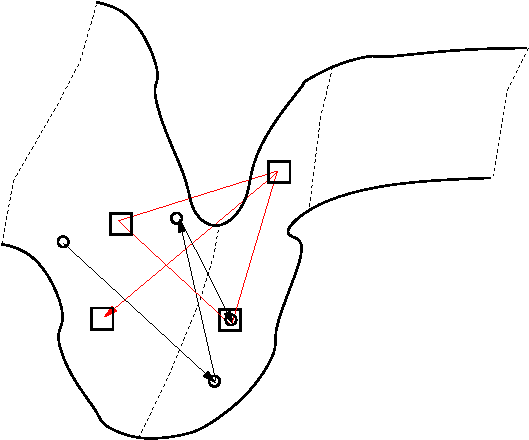
\includegraphics[scale=0.3]{LocalOptima.pdf_t}
\input{LocalOptima.pdf_t}
\caption{Illustration of a situation where the search gets stuck around a local minimum at the bottom of a valley surface representing the cost $\rho$ as function of two-dimensional parameter. The sequence of little circles ($p_1, p_2, p_3, p_4$) represent the sequence of test points generated using Simulated Annealing. Then the Nelder-Mead algorithm is used from $p_3$ and it produces first the triangle (the vertices of which are drawn with little rectangles)  $\{p_4, p_5, p_6 \}$ and then creates a new vertex $p_7$ by reflection. It can be seen that even switching between these two solvers, it is not possible to escape the ``valley'' around this local minimum, and an exploration-driven search is needed.} 
\end{figure}

\section{Solver Initialization}\label{sec:init}

In this section, we describe the $InitialPointSelection$ function in Algorithm \ref{algoSolverExpl}, which selects initial parameter points for a solver. We propose three heuristics to do so:
\begin{itemize}
\item The first way is to select an initial point or a population of initial points from the best points obtained from previous iterations, and repeat this process until achieving a satisfying result. Although different solvers are used, such a greedy method can still lead to a blocking state. 
\item Using an exploration-based approach, we can uniformly sample points over the parameter space, which is essentially what the above-mentioned pseudorandom sampling method does. This, however, does not allow an iteration to exploit the results of the previous iterations. 
\item The third heuristic is to pick initial parameter points according to a distribution that is dynamically updated based on the previous results. This idea, inspired by the population based methods such as the CMA-ES, is described in the sequel. 
\end{itemize}
\subsection{Iteratively updated initial point sampling distribution}
As described above, after each iteration we keep the points visited in the previous iterations. In each iteration we select a set $\mathcal{B}$ of best points, the robustness values of which are below some threshold, and use them to define the sampling distribution for new candidates. 
%The iterative sampling process can be summarized by three steps in the $k^{th}$ iteration: 
%\begin{itemize}
%\item sample $N^k$ candidates based on a probability model; 
%\item evaluate the sampled candidates; 
%\item update the probability model for the sampling process in the next round.
%\end{itemize}
Let $\param \in \real^n$ be a parameter point, let $\param_i$ denote its $i^{th}$ coordinate. For any point $\param$ in $\mathcal{B}$, let $[\underline{\param}_i, \overline{\param}_i]$  be the bounding interval such that each coordinate $\param_i \in [\underline{\param}_i, \overline{\param}_i]$. In the $k^{th}$ iteration, the sampling distribution of $\param_i$ can be a normal distribution $\mathcal{N}(\overline{\param}^k_i, \sigma_i^k)$, where the mean $\overline{\param}^k_i$ is one of the most promising candidates from the previous iteration, selected based on the robustness value. The standard deviation $\sigma_i^k$ in the $k^{th}$ iteration can be determined by: 
\begin{equation} \label{eq:sigma}
\sigma_i^k = (\overline{\param}_i - \underline{\param}_i) (\frac{1}{N^k})^{k/n}
\end{equation}
which decreases iteration after iteration. The number $N^k$ of candidates can vary, being large at the beginning and decreasing gradually. In the first iteration where no information is available, we can sample candidate parameter points according to a uniform distribution. 


\subsection{Keeping promising points}
A point visited by one solver can be a starting point for solvers used in subsequent iterations. \textcolor{red}{Note that we may run a solver multiple again but only from the best points from the previous runs of this solvers because the solvers tend to produce the same results for the same initial points unless their settings are modified. <-- I don't understand; can we just kill this sentence?} Running a solver from the points visited by the other solvers can make the set of visited states quickly become large. Thus, we keep only {\em promising} points. Note that a promising point is not necessarily among the best points. It is simply a point that is still worth being kept. To this end, we will make use of a well-known method for tuning algorithm configurations, called F-Race \cite{Birattari2010}, which was inspired from racing algorithms in machine learning. F-Race is used to evaluate a given set of algorithm configurations iteratively on a sequence of problem instances. When there is sufficient statistical indication that a configuration performs poorly, it is excluded from the future search process. %To do so, the F-Race method employs Friedman test \cite{GVK24551600X}. 
%In the following we show how this idea can be applied to our problem of solver initialization.
%To find appropriate initial points for the solvers, we inspire from the algorithm configuration tuning methods.  These methods essentially determine the best configurations of an algorithm (designed to solve a given problem) based on the results of running the algorithm on a set of problem instances. The configurations with best performance (with respect to some criteria) will then be used for new problem instances (that arise in the future), since an underlying assumption this approach relies on is that the set of considered instances represent sufficiently well the set of all the possible instances.  
In our falsification setting, we will use these concepts with slightly different meanings. Indeed, we have only one problem instance (defined by a dynamical system and a property), but a number of available solvers; however, we follow the spirit of the algorithm configuration tuning approach, by letting solver initial points play the role of algorithm configurations.

%The solver initialization problem can be formally defined by the following elements
%\begin{itemize}
%%\item $\Gamma$ is the set of parameter values.
%\item $\solversetall$ is the set of solvers.
%%\item $\pi_I$ is a probability measure over the set $I$.
%\item $\exectime : \solversetall \to \real_+$ is a function associating to each solver of index $\solver$ an execution time.
%\item $c(\param, \solver)$ is a variable representing the cost function value obtained by running the solver $\solver$ from the point $\param \in \paramset$. 
%\item $C \subset \real$ is the set of possible cost values for all configurations $\theta \in \Theta$ and $\iota \in I$.
%\item $\pi_C$ is a probability measure over the set $C$. Thus $\pi_C(c ~|~ \theta, \iota)$ is the probability that $c$ is the cost of running configuration $\theta$ on instance $\iota$.
%\item $C(\theta) = C(\theta ~|~ \Theta, I, \pi_I, \pi_C, t)$ is the criterion that needs to be optimized with respect to $\theta$. In the most general case it measures in some sense the desirability of the configuration $\theta$.
%\item $T$ is the total amount of time available for experimenting with the given candidate configurations on the available instances before delivering the selected configuration.
%\end{itemize}
%In other words, let $c(\param, \solver)$ be the minimal robustness value (over the output traces and with respect to the property $\spec$) obtained by executing the solver $\solver$ from the point $\param$. 

Let $c(\param, \solver)$ be a variable representing the cost function value obtained by running the solver $\solver$ from the point $\param \in \paramset$. Note that $c(\param, \solver)$ can be thought of as a random variable because of the randomized elements in some solvers. 
%\begin{equation}
%min \{  \rho(\spec, \behaviorfunc(\param)) ~|~ \param \in \paramset \} 
%\end{equation}
%where $\rho(\spec, \behaviorfunc(\param))$ denotes the robustness of the output trajectory $\behaviorfunc(\param)$ with respect to the property $\spec$. The output signal $\behaviorfunc(\param)$ is obtained under the parameter $\param$. 

%Our solver initialization problem can thus be thought of as searching for an initial parameter value that leads a solver to minimize the objective function $c$. 

%Let $\mathcal{A}$ be the set of search algorithms (such as Simulated Annealing, CMAES, etc.) that are available to us. Mapping to the terminology of the algorithm tuning context, 
% \begin{itemize}
% \item a search algorithm $A \in \mathcal{A}$ (together with one of its internal settings) is an instance in the algorithm tuning terminology. As an example of internal settings of a search algorithm, if the search method is Simulated Annealing, a setting is defined by the initial temperature, the number of iterations on one temperature stage and the temperature cooling rate.  
%\item a {\em configuration} (in the algorithm tuning terminology) is a parameter value $\theta \in \Theta$ at which a search algorithm starts. 
%\item If the specifications of interest are expressed by STL \cite{STL} formulas, $c(\theta, A, t)$ is the minimal robustness value over the simulation traces that the configuration (parameter) $\theta$ generates after running for $t$ time using the algorithm instances (algorithm and one of its setting).
%\end{itemize}
%The measures $\pi_I$ and $\pi_C$ in general are not known, the expected cost is estimated in a Monte Carlo fashion by running the falsification algorithm under a configuration on a training set of instances.




%\subsubsection*{F-Race based algorithm for solver initialization}
%The initial points are then selected from the remaining (more promising) visited points. 
We describe how the F-Race algorithm is integrated into the exploitation procedure to remove from consideration the visited points that are not promising. In the first iteration, no visited points are available, we randomly sample a set of parameter points $\Gamma^0$, which serve as initial candidates. Then, to each candidate, we apply the available solvers for some time and record the corresponding costs. The statistical information from the recorded costs is used to decide if a parameter point is not promising at all and thus is dropped. Suppose again that the current iteration is $k$ and let $\Gamma^k$ be the set of the candidates that are still in the race. Let $m_k = | \Gamma^k | $ be the size of the set $\Gamma^k$. Let $m_s$ be the number of solvers, that is $m_s = | \solversetall|$. The Friedman test assumes that the costs are $m_k$ mutually independent $m_s$-variate random variables. For each solver $\solver$, we construct a cost vector $C^k_s$ which is of size at most $m_k$
\begin{eqnarray}\label{eq:C}
C^k_s = (c_{\solver}(\param^{q_1}), c_{\solver}(\param^{q_2}), \ldots, c_{\solver}(\param^{q_{m_k})})
\end{eqnarray}
Each element of the vector is defined by $c_{\solver}(\param^{q_i}) = c(\param^{q_i}, \solver)$ and corresponds to the best cost obtained by executing the solver $\solver$ from the point $\param^{q_i}$ after a completed run. If a parameter point has not been used with a solver $\solver$, it is not included in the cost vector for the Friedman test but is kept for consideration. The costs $c_{\solver}(\param^{q_i})$ are ranked in non-decreasing order, that is $q_i \le q_{i'}$ if $c_{\solver}(\param^{q_i}) \le c_{\solver}(\param^{q_{i'}})$. For each parameter point $\param^{q_i}$, let $R^{\solver}_{i}$ be the rank of $\param^{q_i}$ with respect to the solver $\solver$. Let $R_{i} =  \sum_{\solver=1}^{m_s} R^{\solver}_{i}$ be the sum of ranks for $\param^i$ ($1 \leq i \leq m_k$) over all the solvers. To perform the Friedman test \cite{GVK24551600X}, we determine
\begin{eqnarray*}
\displaystyle \tau & = \displaystyle{ \frac{ (m_k-1) \sum_{i=1}^{m_k} (R_i - (\frac{m_s(m_k+1)}{2})^2 } {\sum_{s=1}^{m_s} \sum_{i=1}^{m_k}  (R^s_{i})^2 -  \frac{m_s m_k (m_k+1)^2}{4} }}  \nonumber \\ 
\end{eqnarray*}
If the value of $\tau$ is larger than the $(1 - \alpha)$ quantile of the distribution $\chi^2$  with $(m_k - 1)$ degrees of freedom ($\alpha$ is a predefined value), the null hypothesis that all parameter values are equivalent is rejected \cite{AP91}. If at the $k^{th}$ iteration this hypothesis is not rejected, we keep the current set of parameter points. If the null hypothesis is rejected, the candidates with the lowest expected rank are considered the most promising parameter values. We then remove, from the current set, the points with differences in cost beyond some given threshold.  
 %(average ranks are used in case of ties)
 
All the above-described developments lead to a new variant of the falsification algorithm, which uses the heuristic using updated initial point sampling distributions and the F-Race method to retain promising points. This represents one heuristic, though we note that the two first heuristics for initial point selection can also be used in place of this method.%. , which can be used in the $k^{th}$ iteration of Algorithm \ref{algoSolverCombination} instead of Algorithm \ref{algoSolverExpl}. 

 
% \subsubsection*{Iterated F-Race based algorithm for solver initialization}
%The F-Race method can also be iterated as follows. Each iteration corresponds to a round, and in each round a number of candidate parameter values remaining from the previous round are used to bias the sampling of new candidates, in view of sampling around the most promising ones. The iterative F-Race can be summarized by three steps in the $r^{th}$ round: 
%\begin{itemize}
%\item (1) sample $N^r$ candidates based on a probability model; 
%\item (2) evaluate the sampled candidates; 
%\item (3) update the probability model for the sampling process in the next round.
%\end{itemize}
%Let $\param \in \real^n$ be a parameter value of our dynamical system such that each component $\param_i \in [\underline{\param}_i, \overline{\param}_i]$. In the $r^{th}$ round, the sampling distribution of $\param_i$ can be a normal distribution $\mathcal{N}(\overline{\param}^r_i, \sigma_i^r)$, where the mean $\overline{\param}^r_i$ is one of the most promising candidates from the previous iteration, selected using their robustness weights. The standard deviation $\sigma_i^r$ in the $r^{th}$ round can be determined by: 
%\begin{equation} \label{eq:sigma}
%\sigma_i^r = (\overline{\param}_i - \underline{\param}_i) (\frac{1}{N^r})^{r/n}
%\end{equation}
%which decreases iteration after iteration. The number $N^r$ of candidates can vary, being large at the beginning and decreases gradually. In the first iteration where no information is available, we can sample candidates (or parameter values) according to a uniform distribution. The $r^{th}$ round of the procedure is summarized in Algorithm~\ref{algoFals}, which contains the initialization and execution of explotation-driven solvers in the $r^{th} $ round and can replace the "for all solvers"-loop in Algorithm \ref{algoSolverCombination}. 

\begin{algorithm}
\caption{Exploitation in the $k^{th}$ iteration of \ref{algoSolverCombination}}
\caption{$\{ \bestobj, \explostateSet \}=Exploitation(\solversetall, \explostateSet, k)$ \label{algoFRace}}
\begin{algorithmic}
%\Require  
%\Ensure  
%\State $k = 1$
%\State $\Gamma^{k-1}=\emptyset$
%\While{$k \le k_{max}$} 
  \State \Comment{{\em Sample new $N^k$ parameter values using distribution $\pi^k$}}
  \State
  \State $\Gamma  = Sample(\explostateSet, N^{r}, \pi^r)$
   \State
  \ForAll{$\solver \in \solversetRho$} 
   % \State $\Gamma = InitialPointSelection(\explostateSet)$
    \State
     \State \Comment{{\em Run solver $\solver$ from some parameter points in $\Gamma$, if it is not done, for $\exectime_{s}$ time}}    
    % \State \Comment{{\em Some intermediate explored points are added in $\Gamma^k$ to produce the new set  $\Gamma^k$} }   
      \State $\{ \bestobj, \explostateSet \} = Run(\solver, \Gamma, \exectime_{\solver})$   
      \State 
      \State  Update the cost vector $C_s^k$ for these parameter points and their costs in $\explostateSet$ as in (\ref{eq:C})
     %\State $C^k =  C^k \cup c(\Theta^k, A_s, t_{s}^k)$  
     \EndFor
   \State
   \State Run F-Race based algorithm on the cost vectors to exclude the least promising candidates from $\explostateSet$   
   \State
  %\State $k++$  %\Comment{{\em Increment the iteration counter}} 
  \State Update distribution $\pi_i^k=\mathcal{N}(\overline{\param}^k_i, \sigma_i^k)$ for each $i^{th}$ parameter coordinate, using the mean $\overline{\param}^k_i$ and the deviation $\sigma^k_i$ as in (\ref{eq:sigma})
%\If{}
%\ElsIf{ }
%\EndIf
%\EndWhile
\end{algorithmic}
\end{algorithm}



%\begin{verbatim}
%     fprintf(1,'\n Best Robustness Value of this call = %f', new_obj_best);    
%     fprintf(fileID,'\n Best Robustness Value of this call = %f', new_obj_best);
%     
%     if (new_obj_best<=0)
%        fprintf(fileID,'\n Falsifier Found!');
%        
%        comptime = toc(TotCompTime);
%        fprintf(fileID,'\n Exit! TOTAL Computation time = %f seconds',comptime );
%        error('Falisifier found! Exit normally');
%     end
%     
%     
%     if (call_count==1)  
%         min_robustness=new_obj_best;
%         rob_stagnant = false;
%         rob_improved = true;
%         rob_stagnant_count=0; 
%     else    
%         rob_improved = false;
%         if min_robustness > new_obj_best
%            rob_stagnant = false; 
%            rob_change=(min_robustness - new_obj_best)/min_robustness;
%            if (rob_change > rob_epsilon_percent)
%                rob_improved = true;
%            end   
%            min_robustness=new_obj_best;
%         else 
%             if (~(solver_index==0) && ~(solver_index==4))
%                 rob_stagnant_count=rob_stagnant_count+1; 
%             end
%         end
%         
%         if rob_stagnant_count>rob_stagnant_win
%             rob_stagnant = true;
%         end
%         
%     end 
%     
%     fprintf(1,'\n Best Robustness Value so far = %f', min_robustness);   
%     fprintf(fileID,'\n Best Robustness Value so far = %f', min_robustness);
%     
%     
%    robustness_graph_data=...
%        [robustness_graph_data; [total_nb_sim min_robustness]]; 
%  
%    
%    % the coverage graph is monotonic, we check the evolution of coverage
%    % for non-increase by cov_epsilon
%    % recompute current coverage
%    current_coverage_value = Sys.ComputeLogCellOccupancyCoverage; 
%    % update coverage graph data
%    coverage_graph_data= ...
%       [coverage_graph_data; [total_nb_sim current_coverage_value]]; 
%    
%    solver_index_data=[solver_index_data; solver_index]; 
%   
%   
%    fprintf(1,'\n\n\n\n #Call  SolverID  Robustness  Coverage');
%    fprintf(fileID,'\n\n\n\n #Call  SolverID  Robustness  Coverage');
%    fprintf(1,'\nPseudo-random (0), CMA-ES (1), SA (2), GNM (3)');
%    fprintf(fileID,'\nPseudo-random (0), CMA-ES (1), SA (2), GNM (3)');
%    for iii  = 1:call_count
%      fprintf(1,'\n %d  %d  %12.8f  %12.8f',iii, solver_index_data(iii,1),...
%          robustness_graph_data(iii,2),coverage_graph_data(iii,2));
%      fprintf(fileID,'\n %d  %d  %12.8f  %12.8f',iii, solver_index_data(iii,1),...
%          robustness_graph_data(iii,2),coverage_graph_data(iii,2));     
%    end 
%    
%    
%    l = size(coverage_graph_data,1);
%    
%    if (l>cov_monitoring_length)
%        cov_diff = current_coverage_value - ...
%            coverage_graph_data(l-cov_monitoring_length,2);
%        
%        if (cov_diff<cov_epsilon)
%           stagnant_count = stagnant_count + 1; 
%           %coverage does not increases sufficiently
%        else
%           %coverage increases sufficiently
%           stagnant_count=0;
%        end 
%    
%        if (stagnant_count>cov_monitoring_length) 
%            cov_stagnant=true;
%            fprintf(fileID,'\n Coverage stagnant');
%        else
%            stagnant_count=stagnant_count+1;
%        end
%    end
%    
%    % memorizing the previous optimizer
%    if (~(solver_index==0)) 
%        prev_solver_index = solver_index;
%    end  
%    
%    stagnant_count
%    rob_stagnant
%    cov_monitoring_length
%    local_optimum_stuck=(stagnant_count>=cov_monitoring_length) && rob_stagnant
%    
%    
%    if (~local_optimum_stuck)
%        cov_monitoring_length=cov_monitoring_win;
%        PR_duration=0;
%        solver_index = prev_solver_index + 1;
%        
%%             if (solver_index==3) 
%%                 solver_index=1; %skip GNM
%%             end    
%        if (solver_index>(Nb_Optimizers-1)) 
%            fprintf(1,'\n\n*******\n #%d round(s) of solver calls done', round_count);
%            fprintf(fileID,'\n #%d round(s) of solver calls done', round_count);
%            solver_index = 1;
%            round_count = round_count + 1;
%            
%            rob_stagnant
%            
%            if rob_stagnant
%                %strategy_id = 2 %Thao
%                %solver_index=0
%                strategy_id = 0
%            else
%                if rob_improved
%                    strategy_id = 2
%                else 
%                    strategy_id = 1
%                end    
%            end    
%        end
%        
%    else %if local optima stuck
%        solver_index=0; %use pseudorandom sampling to increase coverage
%        PR_duration=PR_duration+1;
%
%        cov_monitoring_length=PR_duration;
%    end 
%    
%    fprintf(1,'\n Solver call %d done', call_count);
%    fprintf(fileID,'\n Solver call %d done', call_count);
%
%end % end of for-loop call_count
%\end{verbatim}

\section{Experimental results}\label{sec:expres}
%% We have implemented our above-described falsification algorithm using
%% the robustness evaluation function implemented in the Breach
%% toolbox~\cite{BreachCAV10}\footnote{We used the latest version
%% available in October 2016, on the
%% site \url{https://people.eecs.berkeley.edu/~donze/breach_page.html}}. In
%% our experiments, we first use two Simulink models having input and
%% output signals and test robustness of STL properties specified on the
%% output signals. These models have been used as benchmarks for
%% evaluating hybrid systems verification and validation techniques. In
%% addition, we also test our approach on an industrial system, which is
%% an air path controller for an automotive fuel cell (FC) application.

In our experiments, we compare the performance of a MATLAB
implementation of the combined metaheuristics algorithm with traditional falsification algorithms. Our implementation uses
the robustness evaluation function together with the following solvers CMA-ES, Simulated Annealing, and Global
Nelder-Mead algorithm implementations integrated in
Breach~\cite{DBLP:conf/cav/Donze10}. 
Our experiments were performed on a computer with 1.4GHz processor with 4GB RAM, running 
MATLAB R2015 64-bit version. 
In the following we first describe the models and the input and parameter settings of the benchmarks. Then we present the experimental results obtained using the new algorithm in comparison with the traditional search techniques used alone. Also, we compare it with a method combining
the CMA-ES and classification \cite{CAV2017}, where in each iteration the visited points are classified in order to identify promising regions.
%The grid used in this method is the same as the grid chosen to define the coverage.  %We will
%call this method as grid based random sampling, for the sake of
%reference during comparison.


\subsection{Automative Powertrain Control} \label{sec:PTC}
We consider a Simulink model of a closed-loop Automative Powertrain Control
subsystem (PTC). The model contains a representation of an internal combustion engine and an
embedded software controller for the air-to-fuel ratio within the
engine (see~\cite{Dreossi2015} for more details). Here, we
focus on the input-output behavior, considering the
internal model as a blackbox. The model has three input signals,
Pedal Angle, Engine Speed, and Sensor Offset.
The air-to-fuel (A/F) ratio, denoted by $\eta$, is an
output signal for which the following safety requirement was stated
in~\cite{Dreossi2015}: %$\phi = \G_{[5,10]}\lt(\eta<0.5\rt)$.
$\G_{[5,50]}( (\eta[t] < 0.05) \land ( \eta[t] > - 0.05 ))$.
%We allow $\theta$ to take any value in $[0,40]$, while we fix $w=1000$ and $h=1$. 

\paragraph{Input signal settings.}
We consider an input range for
the Pedal Angle as $[0,40]$ and fix the Engine Speed and
Sensor Offset as $1000$ and $1$, respectively. The time horizon is $50$s.  We use  a piecewise constant
signal for the Pedal Angle input, where the signal is parameterized by $10$
uniformly spaced control points in the time horizon.  Thus, we
have a $10$ dimensional search space $\cpset$.% to search for a counterexample of $\phi$.  
%\emph{\textbf {Algorithm setting.}}  For our algorithm, {\bf TODO}
%The global search time is $\Tglobalmax= $ seconds.  
The cell partitioning $\omega$
consists of hypercubes of side length $\epsilon=4$. 
%% The other algorithms, i.e., CMA-ES, uniform random search and Global
%% Nelder-Mead in Breach and S-TaLiRo and run for a
%% maximum time of $5000$s.


\subsection{Automatic transmission} \label{sec:autotrans}
Next, we consider the benchmark model of an Automatic Transmission control
system, which appeared in~\cite{DBLP:conf/cpsweek/HoxhaAF14}\footnote{The model
and property description of this benchmark is available at the site of
the workshop Applied Verification for Continuous and Hybrid Systems,
ARCH 2014-2015, \url{http://cps-vo.org/node/12116}}.  The system has
two input signals, called throttle and brake, respectively, and two
output signals, called the engine speed, denoted $w$ (RPM), and the vehicle
speed, denoted $v$ (mph).%% The specified range
%% in~\cite{FainekosARCH1415} for both the throttle and break inputs was
%% $[0,100]$.

The property states that if the engine speed stays below a value
$\overline{w}$, then the vehicle speed $v$ does not exceed a threshold
$\overline{v}$ within $10$ seconds.  We specify the values of $\overline{w}$ and
$\overline{v}$ to be $2520$ and $50$, respectively, which gives the
following STL property: $\phi=\neg ((\F_{[0,10]}v>50)\wedge(\G w\leq
2520) )$ \cite{DBLP:conf/cpsweek/HoxhaAF14}.

\paragraph{Input signal and parameter settings.}
Initially, the vehicle is at rest, when $v=0$ and $w=0$.  For the
input signals, we consider smaller ranges than specified
in~\cite{DBLP:conf/cpsweek/HoxhaAF14}, which makes the property $\phi$ more
robust.  The throttle signal is allowed to vary between
$[35,100]$ and the brake is allowed to vary between $[0,40]$.  The
time horizon is set to $30$ seconds.  We use piecewise constant input
signals for testing, where the throttle signal is parametrized by $7$
control points and the brake has $3$ control points. Thus, we have a
$10$ dimensional search space.

%\emph{\textbf{Algorithm setting}}.  {\bf TODO}



%\emph{\textbf{Results.}}  {\bf To describe}
%Our algorithm (classification guided
%global search with local search) successfully found a counterexample in
%less than $2000$ seconds for all randomly chosen seeds. As an indication of the 
%number of classification operations that occurred, the final number of separate rectangles
%constructed for while testing the first seed were 31.  In comparison,
%the CMA-ES found a falsifier for two seeds 5000 and 15000 within
%2000 seconds but failed to do so on the other seeds.  The other methods were
%not successful in finding a falsifier within the default stopping time
%of 3000 seconds.  For this example, S-TaLiRo became stuck around a local
%optimum without any significant reduction in robustness value.  The
%results are presented in Table~\ref{tab:results}.  We note that for
%any fixed seed for random sampling, these results are reproducible.


\subsection{Diesel model} \label{sec:diesel} {\bf To describe}

\subsection{Results} 
The results are presented in Table~\ref{tab:results} and Table~\ref{tab:SeedResults}.  We note that for
any fixed seed, that is the index for a sequence of random numbers in MATLAB for random sampling, these results are reproducible. 
As one can see from the tables, our combined metaheuristics algorithm successfully found a counterexample in
less than the time-out limit for all the considered benchmarks and almost for all the seeds. 
The other methods either were not successful in finding a falsifier within the time-out limit or 
took more computation time. Indeed the metaheuristics used alone, in particular Simulated Annealing 
and Global Nelder-Mead, got stuck around local optima for these examples.


\begin{table}[ht]
\caption{Experimental results on the benchmarks with seed 5000}
%\vspace{-0.5em}
%\vspace{-1.5em}
\label{tab:results}
\begin{center}
\begin{tabular}{|c|c|c|c|}
\hline
\multirow{1}{*}{Search method} & \multicolumn{3}{|c|}{Computation time (s)} \\
\hline
\cline{2-4}
 &  PTC & Aut. Trans & Diesel    \\
\hline
\cline{2-4}
 CMA-ES & T.O (5000)  & T.O. (2000)  &  413.252  \\
\hline
\cline{2-4}
 Simulated Annealing &  T.O. (2000) & T.O. (2000)  & TO (2000)     \\
\hline
\cline{2-4}
Global Nelder-Mead &  T.O. (2000) &  TO (2000)  &  TO (2000)    \\
\hline
\cline{2-4}
Pseudo-random & & & \\ 
sampling &  TO (5000)  &  T.O. (2000) & TO (2000)    \\
\hline
\cline{2-4}
Classification + & & & \\ 
CMA-ES  \cite{CAV2017} & 2891  & 2891  & 996    \\
\hline
\cline{2-4}
 Combined + & & & \\ 
 Metaheuristics & 1276.80 &  899.15 & 299.501   \\
\hline
\end{tabular}
\end{center}
{\small T.O.(T): Exceeded indicated time out limit which is $T$ seconds.\\
Property for the PTC model $\phi = \G_{[5,50]}( (\eta[t] < 0.05) \land ( \eta[t] > - 0.05 ))$. \\
Property for the Automatic Transmission model $\phi =  \G(w[t] < 2520) \land  \F_{[0,10]}(v[t] > 50)$. \\
Property for the Diesel Engine model   $\phi = \G_{[5,10]} (Out1[t] < 41.1)$. 
%\emph{Seed}: Index for a sequence of random numbers in MATLAB. \emph{Solver}: Algorithm used for falsification. \emph{Computation time}: Amount of time (in seconds) until falsification or default stopping after the time limit in parentheses. Computation time is reported for a computer with 1.4GHz processor and 4GB RAM, running MATLAB R2015 64-bit version. \emph{Falsification}: Boolean variable indicating whether the algorithm could falsify the property.
}
\end{table}


\begin{table}[ht]
\caption{Experiments with different seeds on the Automatic Transmission benchmark}
%\vspace{-0.5em}
%\vspace{-1.5em}
\label{tab:SeedResults}
\begin{center}
\begin{tabular}{|c|>{\centering\arraybackslash}p{2cm}|>{\centering\arraybackslash}p{1.5cm}|>{\centering\arraybackslash}p{2cm}|>{\centering\arraybackslash}p{1.5cm}|}
\hline
Seed &  \multicolumn{2}{|c|}{Computation time (s)} \\
\hline
\cline{1-1}
 &  Classification + CMA-ES \cite{CAV2017}  & Meta- heuristics  \\
\hline
\cline{1-2}
 0 &   996   &   991.41   \\
\hline
 5000 & 1382   &  899.15   \\
 \hline
10000 &  1720  &  966.87  \\
\hline
15000 &  1355  & 911.55  \\
\hline
\end{tabular}
\end{center}
Property $\phi =  \G(RPM[t] < 2520) \land  \F_{[0,10]}(speed[t] > 50)$. 
% \emph{Solver}: Algorithm used for falsification. \emph{Computation time}: Amount of time (in seconds) until falsification or default stopping after the time limit in parentheses. Computation time is reported for a computer with 1.4GHz processor and 4GB RAM, running MATLAB R2015 64-bit version. \emph{Falsification}: Boolean variable indicating whether the algorithm could falsify the property.}
\end{table}


%% \subsection{Benchmark experiment setup}

%% In our experiment, we try to compare the performance of a MATLAB implementation of our algorithm
%% with the following standard approaches: the uniform random sampling, CMA-ES,
%% Simulated annealing, Global Nelder Mead algorithm implementations (integrated in the same version of the tool 
%% Breach toolbox~\cite{BreachCAV10} that we used for our algorithm implementation), and the S-TaLiRo tool~\cite{TaliroLFS11} by setting Simulated Annealing as optimization algorithm\footnote{We used the latest version available in October 2016, on the site \url{https://sites.google.com/a/asu.edu/s-taliro/home}.}. Our
%% experiments were performed on a computer with 1.4GHz processor with 4GB
%% RAM, running MATLAB R2015 64-bit version. The settings of our algorithm as well as the other
%% falsification algorithm implementations are detailed below.


%% \subsubsection{Input signal specifications} 
%% \emph{Input signal range}.  We considered smaller ranges for
%% input signals than the ranges considered in the earlier
%% papers~\cite{Dreossi2015,FainekosARCH1415}, so that the properties become more robust and
%% consequently difficult to falsify.  F For the Automative Powertrain PTC example,
%% the Pedal Angle range is set as $[0,40]$ and Engine speed and Sensor
%% Offset signals are fixed as $1000$ and $1$, respectively.
%% %=======
%% %In our experiment, we try to compare the performance of our algorithm
%% %with standard approaches like uniform random sampling, CMAES,
%% %Simulated annealing, Global Nelder Mead and the an implementation
%% %distributed with the S-TaLiRo tool. Our
%% %experiments are performed on a computer with 1.4GHz processor with 4GB
%% %RAM.  The experimentes are implemented on MATLAB R2015 64-bit version.
%% %Our algorithm is implemented in the Breach toolbox~\textbf{CITE} for
%% %MATLAB-Simulink.  The setting of our algorithm as well as the other
%% %falsification algorithms is detailed below.
%% %
%% %
%% %\subsubsection{Input signal specifications} 
%% %\emph{Input signal range}.  We considered smaller ranges for input
%% %signals than the ranges considered in the earlier papers~\cite{todo},
%% %so that the properties become more robust and consequently difficult
%% %to falsify.  For the Automatic Transmission example, the throttle
%% %signal is allowed to vary between $[35,100]$ and the break is allowed
%% %to vary between $[0,40]$. For the Automative Powertrain PTC example,
%% %the Pedal Angle range is set as $[0,40]$ and Engine speed and Sensor
%% %Offset signals are fixed as $1000$ and $1$, respectively.
%% %>>>>>>> efa2003730ca38787c30f35819df6ca0f14cfe20

%% \emph{Finite parametrization of input signals.} We consider
%% piecewise constant input signals.  Furthermore, the allowed time
%% points of discontinuity for the piecewise constant signals are
%% uniformly spaced in the simulation time range of the signals.  For the
%% Automatic Transmission example, the throttle signal has $7$ control
%% points and the break signal has $3$ control points. So, we have
%% $m=7+3=10$ dimensional parameterized input signal space $\cpset$.  For the
%% Automative Powertrain Control example, we have $10$ control points,
%% thus, $\cpset$ is a $10$-dimensional space.


%% \subsubsection{Algorithm settings} 
%% \paragraph{Our algorithm setting}
%% \begin{itemize}
%% \item Threshold number of samples of hyperplane classification $K_c$ is
%% $70$ for the Automatic Transmission example and $100$ for the
%% Automative Powertrain Control example. For the Automatic Transmission
%% example, the influence of the break signal is not as much as that of the
%% throttle signal. Hence we considered a smaller threshold for
%% classification compared to the Automative Powertrain Control example.
%% %
%% \item Cell partitioning $\omega$ consists of hypercubes of side
%% length $\epsilon=4$ for both examples.
%% %
%% \item Global search time is $\Tglobalmax=500s$ for Automatic Transmission, while
%% $\Tglobalmax=2000s$ for the Automative Powertrain Control example.  The
%% Automative Powertrain example has a higher global search time because
%% the time of each function evaluation (simulation) is higher.
%% \item Local search settings. The CMA-ES implementation from
%% Breach-MATLAB toolbox was run for $4$ random number generating seeds: $0$,
%% $5000$, $10000$ and $15000$. The maximum time for the algorithm is
%% set to $2000$s for Automatic Transmission example and $5000$s for Automative Powertrain Control example.
%% \end{itemize}



%% \paragraph{S-TaLiRo setting.}  The Automatic transmission example is available in the distribution of
%% S-TaLiRo\footnote{The used distribution is available at~\url{sites.google.com/a/asu.edu/s-taliro/s-taliro/download}}.
%% For our experiment, we run the script provided in the distribution
%% with the following changes and specifications.  The range of throttle
%% input is reduced to $[35,100]$, while the original script specified
%% it as $[0,100]$.  The break input range is reduced to $[0,40]$, while
%% the original script has the range $[0,40]$.  We changed the class of
%% signals to piecewise constant.  Furthermore, we set the system to be a
%% black box, by setting the relevant S-TaLiRo options.  For the property
%% $\phi$, the script requires values for $\overline{\omega}$
%% and $\overline{v}$.  We specified them as $2520$ and $50$
%% respectively, according to the property we considered in the example.
%% The maximum number of tests (robustness evaluations) in the experiment
%% is set to $20000$.  The script runs the Simulated annealing algorithm
%% for falsification with the seed zero.  The default seed for random
%% number generation is set to $0$.


%% \paragraph{CMA-ES (in Breach) setting.}  The CMA-ES algorithm from Breach was run with the 
%% following setting.  We set the maximum time for the algorithm to $5000$s. The initialization vector is the mean of the
%% input-range.  We ran the algorithm with $4$ instances of seeds for
%% random number generation, i.e., seeds $0$, $5000$, $10000$ and $15000$.

%% \paragraph{Global-Nelder-Mead (in Breach) setting.} The
%% settings were specified in the default setup of Global-Nelder-Mead in
%% Breach.  The maximum time is set to $5000$ for the Automotive Powertrain and
%% $2000$ for the Automatic Transmission example.

%% \subsection{Benchmark results}  

%% The experimental results for the two benchmarks are reported in Table \ref{tab:results}.


%% For the Automatic Transmission example, just the global search phase
%% of our algorithm, i.e., without the CMA-ES local search, successfully
%% found a falsifier within $1000$s. In comparison, the CMA-ES algorithm
%% could not falsify within $2000$s for any of these seeds.  The uniform
%% random sampling procedure found a falsifier for only the
%% seed $15000$, but failed to find a falsifier within 2000s for the rest
%% seeds $0$, $5000$, $10000$, and $20000$.  Also, the Global Nelder Mead and
%% Simulated Annealing could not falsify within $2000$s and S-TaLiRo could
%% not falsify within $3000$s.

%% For the Automative Powertrain Control example, our algorithm successfully found
%% a falsifier within $3000$s for all the seeds.  This involved running
%% the global search phase for $2000$s followed by the CMA-ES local search
%% (until falsification).  However, the CMA-ES search alone, without
%% initialization guidance from hyperplane classification, could not
%% falsify within $5000$s for any of the above seeds.  The uniform random
%% sampling algorithm found a falsifier only for the seeds $10000$ and
%% $15000$, but failed to find falsifier within $5000$s for the rest seeds
%% $0,5000$ and $20000$.  The Global Nelder Mead and Simulated annealing
%% also could not falsify within $5000$s.


%\vspace{-1em}
%\subsection{Industrial example} 
%\input{FCexample.tex}

\section{Related Work}
Our approach is inspired by the hybrid metaheuristics resulting from a hybridization of different metaheuristics, or hybridization of metaheuristics with some heuristics (see a survey \cite{Talbi2009}, the books \cite{Lones2011,Talbi2013} and abundant references therein). The overall goal of such hybridizations is to combine the strengths of exploitation and exploration. A hybridization can be at a component level, that is some component of a metaheuristics is replaced by a metaheuristic. For example, inside an Evolutionary Algorithm the mutation operator can be performed by a local search algorithm. A hybridization can be at a higher level, that is the internal components of the metaheuristics are unchanged, but they are executed sequentially, each using the results of the previous ones. One example is when an exploitation-driven search is run for each individual inside a population-based method in order to improve the population. Our approach indeed belongs to this high level hybridization category. However, in most the existing hybrid algorithms, the hybridization is not adaptive to the current search situation, as in our approach. The reason is that the hybridization aims only at improving some functionalities or elements of each metaheuristic, or sequential execution of metaheuristics is predefined based only on a fixed computation limit for each execution or on exploitation performance (whether the cost value is improved). For example, an exploitation-driven, such as Hill Climbing or Simulated Annealing can have a random restart after running for some fixed amount of time. Our approach additionally uses a global assessment of exploration performance, in terms of coverage measures, to detect important qualitative behavior of the search (in particular entering a basin of attraction around a local optimum) and to make decision on which metaheuristic to execute next. Our notion of coverage is close in spirit to the notion of diversity in population-based methods to determine how similar individuals are. This notion is used in scatter search \cite{Glover2011} to reduce the chance of considering individuals which are too close to each other in some metric. In evolutionary algorithms, diversity is also used in fitness sharing ttechniques o add a penalty on similarity in the fitness function, or in crowding techniques to select individuals to eliminate or to be replaced by their fitter chidren \cite{WongWMPZ2012}. We note that while diversity metrics are used in internal functioning of these methods, our coverage measure is used in a higher level to monitor the overall search progress.


To conclude, we have presented a new falsification algorithm based on a combination of different metaheuristics that exploits their complementary properties. It also integrates a method for timed pattern generation to better handle input signal spaces subject to temporal constraints.
The metaheuristics combination is guided to enhance both exploitation performance, measured by robustness, and exploration performance measured by coverage. This allows the falsification algorithm to converge faster while being able to escape local optima. 
We demonstrated the efficiency of the new algorithm by falsifying
properties on a number of benchmarks, for which this algorithm outperformed some existing algorithms. Ongoing work includes considering the usage of other coverage measures, such as combinatorial entropy. 


\bibliographystyle{plain}
\bibliography{bibliography} 
\end{document}
